% homework/hw06/hw06.tex
% Year 7 - Homework Packet 6: Unit 2, both subjects, and the place they meet.
%
% Covers Mathematics 2.1-2.2 (constructing expressions; using expressions and
% formulae) and Science 2.1-2.2 (solids, liquids and gases; particle theory;
% changes of state; measuring volume and temperature).
%
% SECTION C IS THE POINT OF THIS PACKET. Volume is the one quantity both
% subjects handed this class in the same week, from opposite ends: Science
% measured it in a cylinder in cm^3, Maths built it out of letters. Section C
% puts them together on one idea --
%
%     the small number in the unit counts how many lengths you multiplied
%
% so cm, cm^2 and cm^3 stop being three unrelated labels to memorise and become
% one letter, two letters, three letters. Everything in C follows from that:
% V = lwh is three lengths; 2l + 2w is a sum of lengths and is therefore still
% cm; a tank with a fixed base turns a depth into the expression 300h; and the
% science property "a liquid keeps its volume but takes the shape of its
% container" becomes the algebraic statement that l, w and h all change while
% lwh does not. C4 does the same for a gas, where the volume DOES change,
% because the gaps between the particles close.
%
% Nothing here is lifted from the workbook. Where a trap from the deck is
% reused it has new numbers and a new context.
%
% House style is shared: see homework/hw-style.tex. Method: the new-homework
% skill. Source is pure ASCII on purpose.
%
% Build:  pwsh .claude/skills/new-homework/scripts/build-hw.ps1 hw06

\documentclass[12pt,a4paper]{article}

% -- Answer key switch -------------------------------------------------------
\newif\ifkey
\ifdefined\TEACHER\keytrue\else
  \keyfalse        % \keyfalse = student copy   |   \keytrue = teacher copy
\fi

% -- House style -------------------------------------------------------------
% homework/hw-style.tex
% Shared house style for every Year 7 homework packet. \input this from the
% packet file, right after \documentclass and the answer-key switch.
%
% Do not fork this file per packet. If a packet needs a different look, the
% question is whether every packet should have it.
%
% The choices here are deliberate and were arrived at by printing and looking:
%   * No solid dark banners. Every header is a light tint with a coloured spine
%     on the left, so colour reads clearly without flooding a school printer.
%   * No marks and no mark totals. These are practice, not exam papers.
%   * Lato at 12pt with open leading, plus mathastext so inline maths is Lato
%     too. Without mathastext every "-6 + 4" is Computer Modern serif and the
%     sheet looks half-typeset.
%   * Writing lines are spaced for Year 7 handwriting, not adult margin notes.
%
% Provides: \wlines \blank \tickbox \sep \qmk-free marks (none) \hwsection
% \qhead \expr, the workspace box, and the remember / wordhelp / activity /
% yourturn coloured boxes. Palette matches the lesson decks exactly.

% -- Packages ----------------------------------------------------------------
\usepackage[T1]{fontenc}
\usepackage[utf8]{inputenc}
\usepackage[default]{lato}
\usepackage[a4paper,top=1.7cm,bottom=1.7cm,left=2.0cm,right=2.0cm,headheight=15pt]{geometry}
\usepackage{amsmath,amssymb}
\usepackage{xcolor}
\usepackage[most]{tcolorbox}
\usepackage{enumitem}
\usepackage{tikz}
\usetikzlibrary{arrows.meta}
\usepackage{array}
\usepackage{tabularx}
\usepackage{fancyhdr}
\usepackage{multicol}
\usepackage{needspace}
\usepackage{graphicx}

% Make maths use Lato too. Without this, every "-6 + 4" on the page is set in
% Computer Modern serif and the sheet looks half-typeset. Must come last.
\usepackage[italic]{mathastext}

\linespread{1.06}\selectfont

% -- The Learner's Book palette (same hex values as the lesson decks) ---------
\definecolor{cbteal}{HTML}{0087A8}
\definecolor{cbpurple}{HTML}{5C2483}
\definecolor{cborange}{HTML}{C25E12}
\definecolor{cbgreen}{HTML}{4A8B23}
\definecolor{cbred}{HTML}{C8102E}
\definecolor{cbblue}{HTML}{1A5FA8}
\definecolor{rulegray}{HTML}{9AA5AD}

% -- Answer lines and blanks -------------------------------------------------
% \wlines{n} draws n ruled writing lines, spaced wide enough for Year 7
% handwriting rather than for an adult with a fine pen.
\makeatletter
\newcommand{\wlines}[1]{%
  \par\vspace{0.75em}%
  \@tempcnta=0\relax
  \@whilenum\@tempcnta<#1\do{%
    \hbox to \linewidth{\color{rulegray}\leaders\hrule height 0.5pt\hfill}%
    \vspace{1.5em}%
    \advance\@tempcnta by 1\relax}%
  \par\vspace{-0.8em}%
}
\makeatother

% \blank[width] is an inline gap to write a short answer in.
\newcommand{\blank}[1][2.6cm]{\underline{\hspace{#1}}}

% A boxed space for showing working.
\newtcolorbox{workspace}[1][3.4cm]{%
  colback=white, colframe=rulegray, boxrule=0.5pt, arc=5pt,
  height=#1, left=6pt, right=6pt, top=4pt, bottom=4pt,
  before skip=9pt, after skip=11pt}

% An empty tick box.
\newcommand{\tickbox}{\fbox{\rule{0pt}{1.15em}\rule{1.15em}{0pt}}}

% A middot separator.
\newcommand{\sep}{\,\textperiodcentered\,}

% -- Section and question headings -------------------------------------------
% Light tint plus a fat coloured spine on the left. No solid dark banner: the
% colour reads clearly but barely costs the printer anything.
% needspace stops a heading stranding alone at the foot of a page. Kept modest:
% too large and it pushes headings over, leaving a worse hole than it prevents.
\newcommand{\hwsection}[2][cbteal]{%
  \needspace{8\baselineskip}%
  \par\vspace{13pt}%
  \noindent
  \begin{tcolorbox}[enhanced, nobeforeafter, width=\textwidth,
      colback=#1!7, colframe=#1!7, arc=5pt,
      borderline west={5pt}{0pt}{#1},
      left=14pt, right=10pt, top=7pt, bottom=7pt]
    {\large\bfseries\color{#1}#2}
  \end{tcolorbox}%
  \par\vspace{9pt}}

% \qhead[colour]{A2}{Moving along the line} -- a question heading.
\newcommand{\qhead}[3][cbteal]{%
  \needspace{6\baselineskip}%
  \par\vspace{11pt}%
  \noindent{\large\bfseries\color{#1}#2}\quad{\large\bfseries #3}\par\vspace{4pt}}

% -- Coloured boxes ----------------------------------------------------------
% Shared look: rounded, light fill, coloured rule, coloured title text on a
% pale title strip rather than a dark one.
\tcbset{hwbox/.style={
  enhanced, breakable, arc=6pt, boxrule=1pt,
  left=11pt, right=11pt, top=8pt, bottom=8pt,
  fonttitle=\bfseries, attach boxed title to top left={xshift=12pt, yshift=-8pt},
  boxed title style={arc=4pt, boxrule=1pt, left=7pt, right=7pt, top=2pt, bottom=2pt},
  top=13pt}}

% Orange: things to remember. Matches the deck's "Write This Down".
\newtcolorbox{remember}[1][Remember from the lesson]{hwbox,
  colback=cborange!6, colframe=cborange, coltitle=cborange,
  colbacktitle=white, title={#1}}

% Blue: English help. The barrier in this class is the wording, not the maths.
\newtcolorbox{wordhelp}[1][Word help]{hwbox,
  colback=cbblue!6, colframe=cbblue, coltitle=cbblue,
  colbacktitle=white, title={#1}}

% Purple: an activity or instruction.
\newtcolorbox{activity}[1][How to do this homework]{hwbox,
  colback=cbpurple!6, colframe=cbpurple, coltitle=cbpurple,
  colbacktitle=white, title={#1}}

% Green: your turn / a friendly nudge.
\newtcolorbox{yourturn}[1][Your turn]{hwbox,
  colback=cbgreen!7, colframe=cbgreen, coltitle=cbgreen!75!black,
  colbacktitle=white, title={#1}}

% -- Shorthands --------------------------------------------------------------
\newcommand{\dC}{\,^{\circ}\mathrm{C}}          % use inside maths: $-8\dC$
\newcommand{\key}[1]{{\color{cborange}\textbf{#1}}}
\newcommand{\eng}[1]{{\color{cbblue}\textbf{#1}}}

\setlist[enumerate]{itemsep=8pt, topsep=5pt, leftmargin=*}
\setlist[itemize]{itemsep=4pt, topsep=4pt, leftmargin=*}
\renewcommand{\arraystretch}{1.45}

% -- An expression the student is asked to work from -------------------------
\newcommand{\expr}[1]{%
  \tcbox[on line, colback=cbgreen!10, colframe=cbgreen!55, boxrule=1pt, arc=4pt,
         left=9pt, right=9pt, top=4pt, bottom=4pt]{\large\bfseries $#1$}}

% -- Running head and foot ---------------------------------------------------
% The packet overrides \fancyhead[L] with its own title.
\pagestyle{fancy}
\fancyhf{}
\fancyhead[L]{\small\color{black!55}Year 7\sep Homework}
\fancyhead[R]{\small\color{black!55}Name: \blank[3.4cm]}
\fancyfoot[C]{\small\color{black!55}Page \thepage}
\renewcommand{\headrulewidth}{0pt}
\renewcommand{\headrule}{\vspace{2pt}\hbox to\headwidth{\color{cbteal!45}\leaders\hrule height 1.2pt\hfill}}



% -- Per-packet running head -------------------------------------------------
\fancyhead[L]{\small\color{black!55}Year 7\sep Homework 6}

% -- A group of writing lines that will not be split -------------------------
% \wlines is a run of separate \hboxes, so TeX will happily break in the middle
% of one and strand a single rule at the top of the next page. It did, three
% times, before this existed. n+1 baselineskips is a shade more than n lines
% actually occupy -- enough to keep the group whole, small enough not to push
% the question over and open a bigger hole than it prevents.
\newcommand{\qlines}[1]{\par\needspace{\numexpr#1+1\relax\baselineskip}\wlines{#1}}

% -- A note on the word-help tables ------------------------------------------
% Both of them are written {@{}l@{\hspace{16pt}}X@{}}, spelled out in full.
%
% The first column must be `l', not `p'. LaTeX inserts the stretched row strut
% into the FIRST cell only, and inside a p-column that strut lands in the
% parbox and pushes the text down a line, so every left-hand phrase printed one
% line below the meaning it belonged to.
%
% Do not try to hide the spec behind a macro or the table behind a wrapper
% environment. array does not expand macros in a preamble spec ("Illegal
% pream-token"), and tabularx reads ahead for a literal \end{tabularx}, so a
% wrapper environment breaks it outright. Both were tried.

\begin{document}

% ===========================================================================
% COVER BLOCK
% ===========================================================================
\thispagestyle{fancy}

\begin{tcolorbox}[enhanced, colback=cbpurple!7, colframe=cbpurple!7, arc=7pt,
                  borderline west={6pt}{0pt}{cbpurple},
                  left=18pt, right=14pt, top=10pt, bottom=10pt]
  {\color{cbpurple}\bfseries YEAR 7\sep UNIT 2\sep HOMEWORK 6}\\[5pt]
  {\color{cbpurple}\Huge\bfseries Letters and Particles}\\[7pt]
  {\color{black!70}Mathematics 2.1--2.2 --- expressions, formulae and substituting}\\
  {\color{black!70}Science 2.1--2.2 --- states of matter, particles, changes of state}\\
  {\color{black!70}Section C --- the one thing both subjects measured this week}
\end{tcolorbox}

\vspace{4pt}
\noindent
\begin{tabularx}{\textwidth}{@{}X X@{}}
  \textbf{Name:} \blank[5.6cm] & \textbf{Class:} \blank[5.6cm] \\
  \textbf{Date given:} \blank[4.6cm] &
  \textbf{Date due:} {\color{cbred}\bfseries Monday 14 September 2026} \\
\end{tabularx}

\vspace{2pt}
\begin{activity}
  Three sections. Maths first, then science, then \key{Section C}, where the two
  meet.
  \begin{itemize}
    \item In maths, \key{write the middle line} --- put the times signs back in
          first. And remember that $c-50$ is a \key{finished answer}: you are
          allowed to stop.
    \item In science, answer in \key{full English sentences}. ``Condensation'' is
          not a sentence; ``This is condensation, from gas to liquid'' is.
  \end{itemize}
\end{activity}

% ===========================================================================
% SECTION A -- MATHEMATICS 2.1-2.2
% ===========================================================================
\hwsection{Section A \textperiodcentered\ Mathematics 2.1--2.2 --- Expressions and Formulae}

% -- A1 ---------------------------------------------------------------------
% The way in, and it is meant to be easy: two definitions, eight items, tick a
% column. A student who cannot start anything else can start this.
% The instruction line comes BEFORE the box, not after it. A section heading
% followed immediately by a big tcolorbox cannot be broken apart, so the pair
% moved to page 2 and left the cover page two-thirds empty. One line of prose
% between them gives TeX somewhere to break and buys back most of a page.
\qhead{A1}{Expression, formula, or neither?}

\noindent Tick one box in each row. The first one is done for you.

\begin{remember}[The two definitions, side by side]
  An \key{expression} contains letters and sometimes numbers, and has
  \key{no equals sign}. \quad For example: $n+7$, \; $4m$, \; $x-3$.

  \smallskip
  A \key{formula} is a rule connecting two or more quantities. It contains
  letters and \key{has an equals sign}. \quad For example: $A = lw$, \; $y = 5x$.
\end{remember}

\vspace{6pt}
\noindent
\begin{tabularx}{\textwidth}{|X|c|c|c|}
  \hline
  & \textbf{Expression} & \textbf{Formula} & \textbf{Neither} \\
  \hline
  $6h$ \rule[-0.65em]{0pt}{2.0em}            & \textbf{X} & & \\ \hline
  $P = 4s$ \rule[-0.65em]{0pt}{2.0em}        & & & \\ \hline
  $8 + 5 = 13$ \rule[-0.65em]{0pt}{2.0em}    & & & \\ \hline
  $t - 9$ \rule[-0.65em]{0pt}{2.0em}         & & & \\ \hline
  $V = lwh$ \rule[-0.65em]{0pt}{2.0em}       & & & \\ \hline
  $m = 4 + n$ \rule[-0.65em]{0pt}{2.0em}     & & & \\ \hline
\end{tabularx}

% -- A2 ---------------------------------------------------------------------
\qhead{A2}{Write the expression}

\noindent Mr Bowen has a beaker holding \textbf{$w$ grams} of salt. Write an
expression for the mass of salt in each of these.

\begin{wordhelp}[Word help --- the phrases, and the two that decide the operation]
  \begin{tabularx}{\linewidth}{@{}l@{\hspace{16pt}}X@{}}
    \eng{more than} \sep \eng{fewer than}   & add \sep subtract \\
    \eng{times as many / as much}           & multiply \\
    \eng{half as much}                      & divide by 2 \\
    \eng{the total of}                      & add them together \\
    \eng{the difference between}            & subtract the smaller from the larger \\
  \end{tabularx}

  \smallskip
  Write $3 \times s$ as \key{3s}, and $s \div 2$ as \key{s over 2}. The number
  always goes \key{in front} of the letter --- never $s3$.
\end{wordhelp}

% One column, not two. In two columns these items wrap and the answer blank
% falls onto a line of its own, and the justification stretches "30 grams more
% than Mr Bowen" across the whole column.
\begin{enumerate}[label=(\alph*), itemsep=8pt]
  \item 30 grams more than Mr Bowen \hfill \blank[3.0cm]
  \item Four times as much as Mr Bowen \hfill \blank[3.0cm]
  \item 25 grams fewer than Mr Bowen \hfill \blank[3.0cm]
  \item Half as much as Mr Bowen \hfill \blank[3.0cm]
\end{enumerate}

\vspace{4pt}
\noindent Now two beakers. The first holds $p$ grams and the second holds $q$ grams.
Write an expression for:

\vspace{2pt}
\begin{enumerate}[label=(\alph*), start=5, itemsep=8pt]
  \item the \eng{total} mass of salt in the two beakers \hfill \blank[3.0cm]
  \item the \eng{difference} between the two masses \hfill \blank[3.0cm]
  \item the mass in \textbf{six} beakers like the first and \textbf{two} like the
        second \hfill \blank[3.0cm]
\end{enumerate}

% -- A3 ---------------------------------------------------------------------
% The protected question. Nothing here is new arithmetic; all of it is reading.
\qhead{A3}{The word that changes the order}

\begin{wordhelp}[Word help --- read these twice before you start]
  \begin{tabularx}{\linewidth}{@{}l@{\hspace{16pt}}X@{}}
    \eng{subtract 6}          & you take 6 away from what you have: \; $4x - 6$ \\
    \eng{subtract from 6}     & you \textbf{start} at 6 and take away what you have: \; $6 - 4x$ \\
    \eng{h less than t}       & you start at $t$: \; $t - h$. The English gives the two letters in the \textbf{opposite order} to the calculation. \\
    \eng{the result}          & the thing you just worked out on the line before \\
  \end{tabularx}
\end{wordhelp}

\noindent Write an expression for each description.

\vspace{4pt}
\begin{enumerate}[label=(\alph*), itemsep=9pt]
  \item Multiply $x$ by 7, then subtract 3. \hfill \blank[3.4cm]
  \item Multiply $x$ by 7, then subtract the result from 3. \hfill \blank[3.4cm]
  \item $g$ less than $k$ \hfill \blank[3.4cm]
  \item $y$ more than nine times $z$ \hfill \blank[3.4cm]
  \item Multiply $n$ by 4, then subtract the result from 30. \hfill \blank[3.4cm]
\end{enumerate}

\vspace{6pt}
\noindent \textbf{(f)} Mr Bowen looks at the expression \expr{9 - 2m} and says:
\emph{``Multiply $m$ by 2, then subtract 9.''}

\smallskip
\noindent Is he right? If he is wrong, write the correct description.
\qlines{2}

% -- A4 ---------------------------------------------------------------------
\qhead{A4}{Substitute --- and put the times sign back in}

\begin{remember}[The middle line]
  $4n$ was only ever a short way of writing $4 \times n$. So when $n = 3$:

  \smallskip
  \hspace*{1.2em}$4n \;=\; 4 \times 3 \;=\; \mathbf{12}$ \qquad
  {\color{cbred}\bfseries not 43.}

  \smallskip
  The middle line is where the marks are. \key{Write it every time.}
\end{remember}

\noindent Work out the value of each expression when $n = 6$. Write the middle line.

\vspace{4pt}
\begin{multicols}{2}
\begin{enumerate}[label=(\alph*), itemsep=11pt]
  \item $n + 8 = \blank[2.6cm]$
  \item $5n = \blank[2.6cm]$
  \item $n - 11 = \blank[2.6cm]$
  \item $\dfrac{n}{2} = \blank[2.4cm]$
\end{enumerate}
\end{multicols}

% -- A5 ---------------------------------------------------------------------
\qhead{A5}{The order of operations does not switch off}

\begin{remember}[Times and divide happen first]
  Even after you have put a number in place of a letter, \key{times and divide}
  still happen \key{before} add and subtract.

  \smallskip
  \hspace*{1.2em}$3x + 2$ \; when $x = 4$ \; is \; $3 \times 4 + 2 = 12 + 2 =
  \mathbf{14}$, \; \textbf{not} 18.
\end{remember}

\noindent Work these out. \key{Show the middle line} --- an answer with no working
cannot be checked.

\vspace{4pt}
\begin{enumerate}[label=(\alph*), itemsep=11pt]
  \item $6x - 5$ \quad when $x = 4$ \hfill \blank[6.4cm]
  \item $30 - 4n$ \quad when $n = 7$ \hfill \blank[6.4cm]
  \item $2a + 3b$ \quad when $a = 5$ and $b = 4$ \hfill \blank[6.4cm]
  \item $\dfrac{k}{3} + 9$ \quad when $k = 24$ \hfill \blank[6.4cm]
\end{enumerate}

% -- A6 ---------------------------------------------------------------------
\qhead{A6}{The minus sign travels with its number}

\begin{remember}[Use brackets]
  When the number you are substituting is \key{negative}, put it in
  \key{brackets} so its minus sign cannot be left behind.

  \smallskip
  \hspace*{1.2em}$4 - 3n$ \; when $n = -2$: \quad
  $3n = 3 \times (-2) = -6$, \; so \; $4 - (-6) = 4 + 6 = \mathbf{10}$.
\end{remember}

\noindent Work these out when $m = -5$.

\vspace{4pt}
\begin{multicols}{2}
\begin{enumerate}[label=(\alph*), itemsep=11pt]
  \item $2m = \blank[2.6cm]$
  \item $8 - m = \blank[2.6cm]$
  \item $1 - 2m = \blank[2.6cm]$
\end{enumerate}
\end{multicols}

% -- A7 ---------------------------------------------------------------------
% There was a taxi question here as well -- 12 thousand dong to get in, 8 more
% per kilometre, write C = 12 + 8k. It was cut for the page target, and it was
% the right one to cut: C2 already asks the class to build a formula from a
% described situation, and it does it on a volume, which is where this packet
% is going.
\qhead{A7}{Use a formula}

\noindent Mr Bowen heats a beaker of water. He finds that the temperature in degrees
Celsius is given by the formula

\smallskip
\noindent\hspace*{1.2em}$T = 22 + 6t$, \; where $t$ is the number of minutes since he
lit the burner.

\vspace{4pt}
\begin{enumerate}[label=(\alph*), itemsep=9pt]
  \item Find $T$ when $t = 5$. \hfill \blank[4.4cm]
  \item Find $T$ when $t = 11$. \hfill \blank[4.4cm]
  \item Mr Bowen puts $t = 40$ into the formula and gets $T = 262$. His arithmetic
        is correct. Explain, using what you know from \textbf{Science 2.2}, why the
        water will never reach that temperature.
\end{enumerate}
\qlines{2}

% -- A8 ---------------------------------------------------------------------
\qhead{A8}{Now you write the question}

\begin{yourturn}[Read all four conditions before you start]
  Here is an expression:\qquad \expr{40 - 5n}

  \medskip
  Write a \key{word problem} that this expression is the answer to. Your question
  must:
  \begin{enumerate}[label=\arabic*., itemsep=4pt, topsep=5pt]
    \item be about something \key{real} --- a beaker, money, a journey, a class;
    \item say clearly what \key{n represents};
    \item \key{start} at 40, and take away 5 lots of something;
    \item be written in \key{full sentences} and \key{end in a question}.
  \end{enumerate}
\end{yourturn}

\qlines{4}

% ===========================================================================
% SECTION B -- SCIENCE 2.1-2.2
% ===========================================================================
\hwsection{Section B \textperiodcentered\ Science 2.1--2.2 --- Particles and Changes of State}

% -- B1 ---------------------------------------------------------------------
\qhead{B1}{Match the word to its meaning}

\noindent Write the correct \textbf{letter} in each box.

\vspace{7pt}
\noindent
\begin{tabularx}{\textwidth}{|p{3.6cm}|c|X|}
  \hline
  \textbf{Word} & & \textbf{Meaning} \\
  \hline
  1.\ Matter        & \tickbox & \textbf{A} \; A space with no particles in it at all. \\
  2.\ Property      & \tickbox & \textbf{B} \; Squashed into a smaller space. \\
  3.\ Particle      & \tickbox & \textbf{C} \; The amount of space something takes up. \\
  4.\ Volume        & \tickbox & \textbf{D} \; Everything you can see and feel. \\
  5.\ Compressed    & \tickbox & \textbf{E} \; A tiny piece of matter, far too small to see. \\
  6.\ Vibrate       & \tickbox & \textbf{F} \; A way that a substance behaves. \\
  7.\ Vacuum        & \tickbox & \textbf{G} \; The curved surface of a liquid in a tube. \\
  8.\ Meniscus      & \tickbox & \textbf{H} \; To make tiny movements without leaving your place. \\
  \hline
\end{tabularx}

% -- B2 ---------------------------------------------------------------------
\qhead{B2}{The properties table}

\noindent Put a \textbf{tick} for yes and a \textbf{cross} for no.

\vspace{7pt}
\noindent
\begin{tabularx}{\textwidth}{|X|c|c|c|}
  \hline
  & \textbf{Solid} & \textbf{Liquid} & \textbf{Gas} \\
  \hline
  Keeps its own shape \rule[-0.65em]{0pt}{2.0em}          & & & \\ \hline
  Keeps the same volume \rule[-0.65em]{0pt}{2.0em}        & & & \\ \hline
  Can be poured \rule[-0.65em]{0pt}{2.0em}                & & & \\ \hline
  Can be compressed \rule[-0.65em]{0pt}{2.0em}            & & & \\ \hline
\end{tabularx}

\vspace{9pt}
\noindent \textbf{(b)} Dry sand can be poured from one hand to the other. Sand is
\textbf{not} a liquid. Explain why not.
\qlines{2}

% -- B3 ---------------------------------------------------------------------
\qhead{B3}{Answer in full sentences}

\begin{wordhelp}[Sentence starters --- you may copy these]
  ``In a solid the particles are\ldots'' \qquad
  ``This means that\ldots'' \qquad
  ``\ldots because the gaps between the particles\ldots''
\end{wordhelp}

\noindent \textbf{(a)} You can pour water, but you cannot pour a brick. Use
\eng{particles} to explain the difference.
\qlines{2}

\vspace{4pt}
\noindent \textbf{(b)} Mr Bowen blocks the end of two syringes with his thumb. One is
full of \textbf{air} and one is full of \textbf{water}. Only the air syringe moves when
he pushes. Explain why.
\qlines{2}

\vspace{4pt}
\noindent \textbf{(c)} A kitchen sponge is a solid, but you can squash it in one hand.
Does this prove that particle theory is \textbf{wrong}? Explain your answer.
\qlines{3}

% -- B4 ---------------------------------------------------------------------
\qhead{B4}{The five changes of state}

\noindent Complete the table. The first row is done for you.

\vspace{7pt}
\noindent
\begin{tabularx}{\textwidth}{|p{2.9cm}|p{3.2cm}|X|c|}
  \hline
  \textbf{Doing word} & \textbf{Naming word} & \textbf{From \ldots\ to \ldots} &
  \textbf{Heat or cool?} \\
  \hline
  melt \rule[-0.65em]{0pt}{2.0em}  & melting & solid to liquid & heat \\ \hline
  freeze \rule[-0.65em]{0pt}{2.0em} & & & \\ \hline
   \rule[-0.65em]{0pt}{2.0em} & evaporation & & \\ \hline
  boil \rule[-0.65em]{0pt}{2.0em}  & & & \\ \hline
   \rule[-0.65em]{0pt}{2.0em} & condensation & & \\ \hline
\end{tabularx}

\vspace{9pt}
\noindent \textbf{(b)} Write the two temperatures for water:

\smallskip
\noindent melting point \blank[3.0cm] \qquad boiling point \blank[3.0cm]

% -- B5 ---------------------------------------------------------------------
\qhead{B5}{Evaporating or boiling?}

\begin{remember}[Same journey, different word]
  \key{Evaporation} and \key{boiling} are both liquid to gas. Evaporation is
  \key{slow}, happens at the \key{surface} only, and at \key{any} temperature.
  Boiling is \key{fast}, happens \key{all through} the liquid, and only at the
  \key{boiling point}.
\end{remember}

\noindent Tick one box in each row.

\vspace{6pt}
\noindent
\begin{tabularx}{\textwidth}{|X|c|c|}
  \hline
  & \textbf{Evaporating} & \textbf{Boiling} \\
  \hline
  Washing dries on the line on a cool day \rule[-0.65em]{0pt}{2.0em} & & \\ \hline
  Bubbles form all through the water in a pan \rule[-0.65em]{0pt}{2.0em} & & \\ \hline
  A puddle disappears from the playground \rule[-0.65em]{0pt}{2.0em} & & \\ \hline
  It only happens at $100\dC$ \rule[-0.65em]{0pt}{2.0em} & & \\ \hline
\end{tabularx}

\vspace{9pt}
\noindent \textbf{(b)} Mr Bowen leaves a glass of water on his desk on Friday. On
Monday the glass is empty. The water never reached $100\dC$. Name the change of state
and explain, in full sentences, where the water went.
\qlines{2}

% -- B6 ---------------------------------------------------------------------
% Atomic block: the diagram and its answer lines cannot be split, so it sits at
% the end of Section B where it strands nothing.
\qhead{B6}{Read the scale, then draw one}

\begin{remember}[Both instruments, one rule]
  Read at \key{eye level}. On a measuring cylinder, read the \key{bottom of the
  meniscus}. On a thermometer, read the \key{top} of the liquid.
\end{remember}

\noindent Each small line on the cylinders is $10\ \mathrm{cm^3}$. Write the volume in
\textbf{A} and \textbf{B}, then \textbf{draw} the water level in \textbf{C}.

% y is the height of one 10 cm^3 division. The whole picture is 11.35 of them
% tall and it is ATOMIC -- a tikzpicture cannot be broken -- so its height
% decides which page the block lands on. At 0.64 the block overshot the tail of
% its page by about 1.3 cm and moved whole, costing half a page. Do not enlarge
% it again without re-rendering and counting pages.
\vspace{5pt}
\noindent
\begin{center}
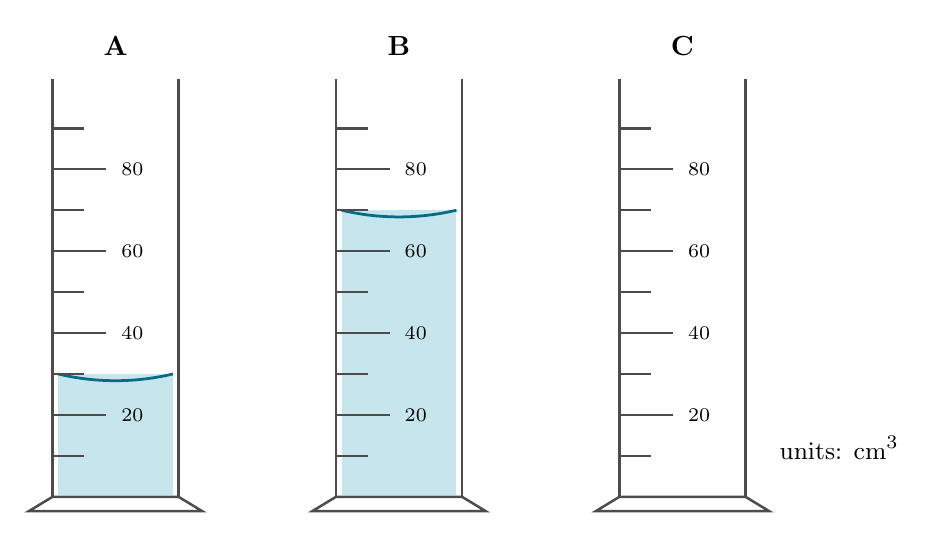
\begin{tikzpicture}[x=1cm, y=0.52cm, line width=0.9pt]

  % -- the empty cylinder, drawn three times. \wv is the water height in tens of
  %    cm^3; 0 means draw no water at all, which is cylinder C.
  %    NOTE: the loop variable must not be called \fill -- that is TikZ's own
  %    drawing command and redefining it breaks every fill on the page.
  \foreach \dx/\wv/\name in {0/3/A, 3.6/7/B, 7.2/0/C}{
    \begin{scope}[shift={(\dx,0)}]
      % water, and the meniscus dipping across the top of it
      \ifnum\wv>0
        \fill[cbteal!22] (0.07,0.05) rectangle (1.53,\wv);
        \draw[cbteal!80!black, line width=1.0pt]
          (0.07,\wv) .. controls (0.55,{\wv-0.22}) and (1.05,{\wv-0.22}) ..
          (1.53,\wv);
      \fi
      % the cylinder body, open at the top, standing on a foot
      \draw[black!70] (0,10.2) -- (0,0) -- (1.6,0) -- (1.6,10.2);
      \draw[black!70] (-0.3,-0.35) -- (1.9,-0.35) -- (1.6,0) -- (0,0) -- cycle;
      % scale: a mark every 10 cm^3, longer and numbered every 20
      \foreach \v in {1,2,...,9}{\draw[black!70] (0,\v) -- (0.40,\v);}
      \foreach \v in {2,4,6,8}{
        \draw[black!70] (0,\v) -- (0.68,\v);
        \node[anchor=west, font=\scriptsize] at (0.74,\v)
          {\pgfmathparse{int(\v*10)}\pgfmathresult};}
      \node[font=\bfseries] at (0.8,11.0) {\name};
    \end{scope}}

  % unit label
  \node[anchor=west, font=\small] at (9.1,1.2) {units: $\mathrm{cm^3}$};

\end{tikzpicture}
\end{center}

\vspace{4pt}
\noindent
\begin{tabular}{@{}p{0.30\textwidth} p{0.30\textwidth} p{0.33\textwidth}@{}}
  \textbf{A} = \blank[2.6cm] & \textbf{B} = \blank[2.6cm] &
  \textbf{C}: draw $45\ \mathrm{cm^3}$ \\
\end{tabular}

\vspace{10pt}
\noindent \textbf{(b)} Two students read cylinder \textbf{A} and get two different
answers. Neither of them misread the numbers. Explain what went wrong.
\qlines{2}

% ===========================================================================
% SECTION C -- THE BRIDGE
% ===========================================================================
\hwsection[cbgreen]{Section C \textperiodcentered\ Where the two subjects meet --- Volume}

\noindent In Science you measured a volume in a cylinder. In Maths you built one out
of letters. They are the same thing, and this section is why.

\begin{remember}[The small number counts the lengths]
  A \key{length} is one measurement: \; $\mathrm{cm}$.

  \smallskip
  An \key{area} is a length \key{times} a length: \; $\mathrm{cm} \times
  \mathrm{cm} = \mathrm{cm^2}$. \; Two lengths, so a small \key{2}.

  \smallskip
  A \key{volume} is a length \key{times} a length \key{times} a length: \;
  $\mathrm{cm} \times \mathrm{cm} \times \mathrm{cm} = \mathrm{cm^3}$. \; Three
  lengths, so a small \key{3}.

  \medskip
  So for a box: \qquad $V = lwh$ \qquad --- three letters multiplied, three
  lengths, $\mathrm{cm^3}$.

  \medskip
  And the unit that joins the two subjects:\qquad
  $1\ \mathrm{cm^3} = 1\ \mathrm{ml}$, \qquad
  $1000\ \mathrm{cm^3} = 1\ \mathrm{litre}$.
\end{remember}

% -- C1 ---------------------------------------------------------------------
\qhead[cbgreen]{C1}{Count the letters}

\noindent Every letter below stands for a length in centimetres. Count how many
lengths are \textbf{multiplied together}, then write the unit. \; The first one is done
for you.

\vspace{7pt}
\noindent
\begin{tabularx}{\textwidth}{|p{3.4cm}|X|p{2.6cm}|}
  \hline
  \textbf{Expression} & \textbf{How many lengths multiplied?} & \textbf{Unit} \\
  \hline
  $h$ \rule[-0.65em]{0pt}{2.0em}       & one & $\mathrm{cm}$ \\ \hline
  $lw$ \rule[-0.65em]{0pt}{2.0em}      & & \\ \hline
  $lwh$ \rule[-0.65em]{0pt}{2.0em}     & & \\ \hline
  $s^3$ \rule[-0.65em]{0pt}{2.0em}     & & \\ \hline
  $2l + 2w$ \rule[-0.65em]{0pt}{2.0em} & & \\ \hline
\end{tabularx}

\vspace{9pt}
\noindent \textbf{(b)} The last row is different from all the others. Explain why the
unit for $2l + 2w$ is \textbf{not} $\mathrm{cm^2}$, even though it has two letters in
it.
\qlines{2}

% -- C2 ---------------------------------------------------------------------
\qhead[cbgreen]{C2}{The tank}

\noindent A tank has a rectangular base measuring $\mathbf{20\ cm}$ by
$\mathbf{15\ cm}$. It is $\mathbf{25\ cm}$ tall. Mr Bowen pours in water to a depth of
$h$ centimetres.

\vspace{8pt}
\begin{center}
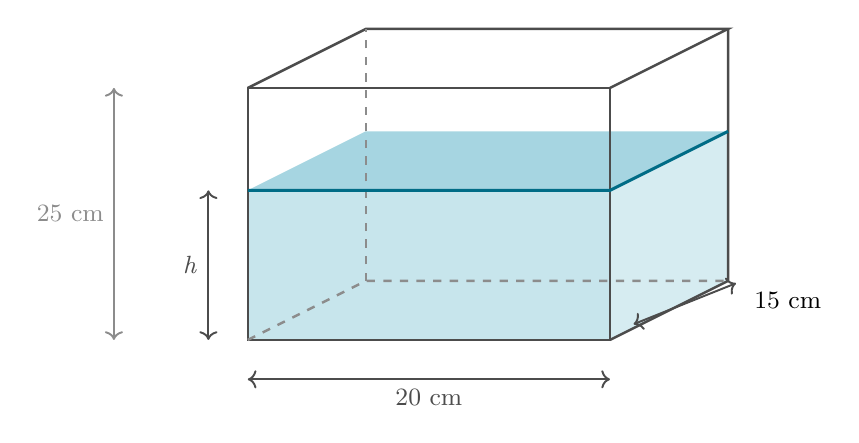
\begin{tikzpicture}[x=1cm, y=1cm, line width=0.9pt]
  % A cuboid tank, part-filled. \tkW/\tkH/\tkD are the drawn width, height and
  % depth; \tkL is the water line. Names are prefixed because \H is a LaTeX
  % accent command and \W is claimed by other packages.
  \def\tkW{4.6} \def\tkH{3.2} \def\tkD{1.5} \def\tkL{1.9}

  % water: front face, then the top surface, then the visible right-hand side
  \fill[cbteal!22] (0,0) rectangle (\tkW,\tkL);
  \fill[cbteal!35] (0,\tkL) -- (\tkD,{\tkL+0.75}) -- ({\tkW+\tkD},{\tkL+0.75})
                   -- (\tkW,\tkL) -- cycle;
  \fill[cbteal!16] (\tkW,0) -- ({\tkW+\tkD},0.75) -- ({\tkW+\tkD},{\tkL+0.75})
                   -- (\tkW,\tkL) -- cycle;

  % tank edges
  \draw[black!70] (0,0) rectangle (\tkW,\tkH);
  \draw[black!70] (0,\tkH) -- (\tkD,{\tkH+0.75}) -- ({\tkW+\tkD},{\tkH+0.75}) -- (\tkW,\tkH);
  \draw[black!70] (\tkW,0) -- ({\tkW+\tkD},0.75) -- ({\tkW+\tkD},{\tkH+0.75});
  \draw[black!45, dashed] (0,0) -- (\tkD,0.75) -- ({\tkW+\tkD},0.75);
  \draw[black!45, dashed] (\tkD,0.75) -- (\tkD,{\tkH+0.75});

  % the water line
  \draw[cbteal!80!black, line width=1.1pt]
    (0,\tkL) -- (\tkW,\tkL) -- ({\tkW+\tkD},{\tkL+0.75});

  % labels
  \draw[<->, black!70, line width=0.7pt] (0,-0.5) -- (\tkW,-0.5)
    node[midway, below, font=\small] {$20$ cm};
  \draw[<->, black!70, line width=0.7pt] ({\tkW+0.3},0.2) -- ({\tkW+\tkD+0.1},0.72);
  \node[anchor=west, font=\small] at ({\tkW+\tkD+0.2},0.5) {$15$ cm};
  \draw[<->, black!70, line width=0.7pt] (-0.5,0) -- (-0.5,\tkL)
    node[midway, left, font=\small] {$h$};
  \draw[<->, black!45, line width=0.7pt] (-1.7,0) -- (-1.7,\tkH)
    node[midway, left, font=\small] {$25$ cm};
\end{tikzpicture}
\end{center}

\vspace{4pt}
\begin{enumerate}[label=(\alph*), itemsep=10pt]
  \item Write an \textbf{expression} for the volume of the water in the tank.
        \hfill \blank[3.4cm]
  \item Write it as a \textbf{formula} beginning $V = $ \hfill \blank[3.4cm]
  \item Find the volume of water when $h = 4$. Show the middle line.
        \hfill \blank[5.0cm]
  \item How many \textbf{litres} of water is that? \hfill \blank[3.4cm]
  \item Mr Bowen substitutes $h = 40$ into his formula and gets
        $12\,000\ \mathrm{cm^3}$. His arithmetic is correct. Explain why the answer
        is still wrong.
\end{enumerate}
\qlines{2}

% -- C3 ---------------------------------------------------------------------
\qhead[cbgreen]{C3}{The same water, three containers}

\noindent Mr Bowen pours the \textbf{same} $150\ \mathrm{cm^3}$ of water from a tall
narrow cylinder into a wide flat dish, and then into a beaker.

\vspace{5pt}
\begin{enumerate}[label=(\alph*), itemsep=10pt]
  \item As the water moves from container to container, which of the three
        measurements --- its \textbf{length}, its \textbf{width}, its
        \textbf{height} --- change? \hfill \blank[4.4cm]
  \item What is the value of $lwh$ in every one of the three containers?
        \hfill \blank[4.4cm]
  \item Complete the science sentence:

        \smallskip
        A liquid keeps the same \blank[3.4cm] but takes the \blank[3.4cm] of its
        container.
  \item So $l$, $w$ and $h$ all change, and $lwh$ does not. Explain in your own
        words how those two facts fit together.
\end{enumerate}
\qlines{2}

% -- C4 ---------------------------------------------------------------------
\qhead[cbgreen]{C4}{The syringe --- where the volume really does change}

\noindent A sealed syringe holds $v\ \mathrm{cm^3}$ of \textbf{air}. Nothing can get in
or out.

\vspace{5pt}
\begin{enumerate}[label=(\alph*), itemsep=10pt]
  \item Mr Bowen pushes the plunger until the air fills \textbf{half} the space it
        did before. Write an expression for the new volume of the air.
        \hfill \blank[3.0cm]
  % There was a part here asking the class to explain, with particles, why a gas
  % compresses and a liquid does not. It is B3(b) -- the two syringes -- almost
  % word for word, so it went. What is left is the pair that only this section
  % can ask: the same push on two substances, one volume halving and one not.
  \item Mr Bowen empties the syringe, fills it with $v\ \mathrm{cm^3}$ of
        \textbf{water} instead, seals it, and pushes just as hard. Write an
        expression for the new volume of the water, and say why.
\end{enumerate}
\qlines{3}

% -- C5 ---------------------------------------------------------------------
\qhead[cbgreen]{C5}{Three bad ideas}

\noindent Mr Bowen has had three ideas. Each one is a bad idea. For each, say
\textbf{what goes wrong}, in a full sentence, using the science or the maths from
this unit.

\vspace{5pt}
\begin{enumerate}[label=\textbf{\arabic*.}, itemsep=11pt]
  \item He wants a smaller cup of tea, so he seals the cup and squeezes it very
        hard.
        \qlines{2}
  \item His formula says the water will be at $262\dC$ after 40 minutes, so he
        plans to leave the burner on and come back at lunchtime.
        \qlines{2}
  \item He measures a box as $10\ \mathrm{cm}$ long, $10\ \mathrm{cm}$ wide and
        $10\ \mathrm{cm}$ tall, and writes that its volume is
        $30\ \mathrm{cm^3}$.
        \qlines{3}
\end{enumerate}

% ===========================================================================
% ANSWER KEY -- TEACHER COPY ONLY
% ===========================================================================
\ifkey
\clearpage

\hwsection[cbred]{Answer Key --- Teacher Copy}

\linespread{1.0}\selectfont
\setlist[enumerate]{itemsep=2pt, topsep=3pt, leftmargin=*}
\setlist[itemize]{itemsep=2pt, topsep=3pt, leftmargin=*}

\qhead[cbred]{A1}{Expression, formula, or neither?}
\noindent $6h$ --- expression \quad $P=4s$ --- formula \quad $8+5=13$ --- neither
\quad $t-9$ --- expression \\
$V=lwh$ --- formula \quad $m=4+n$ --- formula

\smallskip
\noindent{\small The row that separates the class is $8+5=13$. It has an equals sign,
so students who learned ``equals sign means formula'' tick formula --- but it has no
letters, so it is neither. Both halves of each definition have to be checked, and this
row is the only place that shows who is checking one.}

\qhead[cbred]{A2}{Write the expression}
\noindent (a) $w+30$ \quad (b) $4w$ \quad (c) $w-25$ \quad (d) $\dfrac{w}{2}$ \quad
(e) $p+q$ \quad (f) $p-q$ \quad (g) $6p+2q$

\smallskip
\noindent{\small (b) is the one to watch: $w4$ instead of $4w$. The number goes in
front, always, and it is worth correcting on sight rather than in writing. \\
(f) has no single right answer and that is fine --- $q-p$ is equally good, as long as
the student can say which beaker they started at. What is \emph{not} acceptable is
$p+q$, which means the word \emph{difference} was read as ``the answer''. \\
(g) is the two-letter question. A student who writes $8pq$ has merged two different
quantities into one and needs the beakers drawn.}

\qhead[cbred]{A3}{The word that changes the order}
\noindent (a) $7x-3$ \quad (b) $3-7x$ \quad (c) $k-g$ \quad (d) $9z+y$ \quad
(e) $30-4n$

\smallskip
\noindent (f) He is \textbf{wrong}. His description gives $2m-9$. The expression
$9-2m$ starts at 9, so the description needs \emph{subtract the result \textbf{from}
9}.

\smallskip
\noindent{\small (a) and (b) are the same five words with one preposition changed, and
they are printed next to each other on purpose. If a student gives the same answer to
both, they read the numbers and not the sentence --- do not mark it, make them read
both aloud. \\
(c) is $t-h$ with new letters. Check it with numbers if anyone resists: 5 less than 12
is 7, and nobody writes $5-12$ for that. \\
(f) is the best question in Section A after A8, because it runs the translation
\emph{backwards}. A student who cannot spot the error can still often fix it once told
there is one --- that is worth knowing, and it is the difference between not reading
and not being able to.}

\qhead[cbred]{A4}{Substitute}
\noindent (a) $6+8=\mathbf{14}$ \quad (b) $5 \times 6 = \mathbf{30}$ \quad
(c) $6-11=\mathbf{-5}$ \quad (d) $6 \div 2 = \mathbf{3}$

\smallskip
\noindent{\small (b) is the headline error of the whole unit: $\mathbf{56}$, two digits
pushed together, written with total confidence by a student whose arithmetic is
perfect. It is our own fault --- in 2.1 we taught them to write $5 \times n$ as $5n$ --
so treat it as a reading error and put the times sign back in on the board rather than
marking the arithmetic. \\
(c) goes below zero, which is Unit 1 work and is allowed. A student who writes 5 has
decided an answer cannot be negative.}

\qhead[cbred]{A5}{The order of operations}
\noindent (a) $6 \times 4 - 5 = 24-5 = \mathbf{19}$ \\
(b) $30 - 4 \times 7 = 30-28 = \mathbf{2}$ \\
(c) $2 \times 5 + 3 \times 4 = 10+12 = \mathbf{22}$ \\
(d) $24 \div 3 + 9 = 8+9 = \mathbf{17}$

\smallskip
\noindent{\small (b) is the one to slow down on. The multiplication is written
\emph{second} and still happens first; a student working left to right gets
$26 \times 7 = 182$. This is also the shape of C2(e) and of every ``start at 40 and
take away'' question in the unit. \\
Mark the middle line, not the answer. Every error on this question is invisible in a
final number and obvious in the working, which is the entire argument for demanding
it.}

\qhead[cbred]{A6}{The minus sign travels}
\noindent (a) $2 \times (-5) = \mathbf{-10}$ \quad
(b) $8-(-5) = 8+5 = \mathbf{13}$ \quad
(c) $1 - 2 \times (-5) = 1-(-10) = 1+10 = \mathbf{11}$

\smallskip
\noindent{\small (c) is the question. The wrong answer is $\mathbf{-9}$, from
substituting 5 and leaving the minus sign behind. Insist on the brackets at the
substitution step; that one habit fixes the whole class of error. \\
Note that the arithmetic in (c) is $1+10$, and nobody in this room finds that hard.
Say so out loud --- the difficulty is entirely in getting the sign into the expression
in one piece.}

\qhead[cbred]{A7}{Use a formula}
\noindent (a) $T = 22 + 6 \times 5 = 22+30 = \mathbf{52\dC}$ \quad
(b) $T = 22 + 6 \times 11 = 22+66 = \mathbf{88\dC}$ \\
(c) The water \textbf{boils at $100\dC$ and stays there}. The formula describes the
water heating up; once it reaches its boiling point that situation has ended, so the
formula has ended with it.

\smallskip
\noindent{\small \textbf{(c) is the most valuable question in Section A.} The
arithmetic is perfect and the answer is still wrong. If a student says the water would
have boiled away, agree warmly --- they are right, and they have made the point for
you. Anyone who answers ``he did the sum wrong'' has not read the sentence saying he
did not. \\
In (a) and (b), watch for the 22 being multiplied: $6t$ with $t=5$ is 30, and the 22 is
added once, not six times. It is A5's error in a formula.}

\qhead[cbred]{A8}{Now you write the question}
\noindent No single right answer. Check the four conditions \textbf{in this order}:
\begin{enumerate}[label=\arabic*., itemsep=3pt]
  \item \textbf{Does the story start at 40?} It must \emph{begin} there, not arrive
        there. This is the condition most of them will miss.
  \item \textbf{Is it 5 lots of something, repeated?} Five taken away once is not
        $5n$ --- it needs a rate: 5 each day, 5 per person, 5 grams every minute.
  \item \textbf{Is it said what $n$ represents?}
  \item \textbf{Full sentences, ending in a question?}
\end{enumerate}

\smallskip
\noindent{\small One that works: ``A beaker holds 40 grams of salt. Mr Bowen takes out
5 grams every minute. Write an expression for the mass of salt left after $n$
minutes.'' \\
A question that ends ``what is $40-5n$?'' has not done the task --- it is the
expression copied out in words. Name that out loud rather than marking it wrong. \\
This question cannot be answered by pattern-matching, which makes it the single best
thing on the packet for finding out who is reading. Read four or five of them to the
class.}

\qhead[cbred]{B1}{Match the word to its meaning}
\noindent 1--D \quad 2--F \quad 3--E \quad 4--C \quad 5--B \quad 6--H \quad 7--A
\quad 8--G

\smallskip
\noindent{\small \emph{Property} (2--F) is the one that goes wrong, and not because of
the science: the everyday English meaning is a house or land, and a student reaching
for that meaning has nowhere to put F. \\
\emph{Vibrate} (6--H) is the other: it means small movements \textbf{on the spot}, not
travelling. Ask a student to vibrate in their chair without leaving it; it settles in
five seconds.}

\qhead[cbred]{B2}{The properties table}
\noindent
\begin{tabularx}{\linewidth}{@{}Xccc@{}}
  & \textbf{Solid} & \textbf{Liquid} & \textbf{Gas} \\
  Keeps its own shape   & yes & no  & no  \\
  Keeps the same volume & yes & yes & no  \\
  Can be poured         & no  & yes & yes \\
  Can be compressed     & no  & no  & yes \\
\end{tabularx}

\smallskip
\noindent (b) Every \textbf{grain} of sand keeps its own shape and cannot be
compressed, so every grain is a solid. What flows is not one substance pouring --- it
is millions of tiny solids rolling over one another.

\smallskip
\noindent{\small The liquid column is the useful one: it is the only column with a
\emph{yes} and a \emph{no} in the middle two rows, and that pair is exactly what
Section C is built on. Point at it when you mark C3. \\
(b) is a full-sentence question and the sentence matters. ``Because it is a solid'' is
circular; push for the grain.}

\qhead[cbred]{B3}{Answer in full sentences}
\noindent (a) Matter can only flow if the particles can \textbf{move past one
another}. In a solid the attractive forces are strong and hold every particle in its
place. In a liquid the forces are weak enough to let particles slide past each other,
but still strong enough to keep them touching.

\smallskip
\noindent (b) A gas has \textbf{large gaps} between its particles, so pushing simply
moves them closer together and the air takes up less room. In water the particles are
already touching, so there is no gap left to close and the plunger will not move.
Nothing escapes from either syringe.

\smallskip
\noindent (c) \textbf{No.} The sponge is not solid all the way through --- it is a thin
solid skeleton with \textbf{air} in every hole. Squeezing it compresses the air, not
the solid, and the air pushes it back when you let go.

\smallskip
\noindent{\small (c) is the best question in Section B and should be discussed rather
than marked. It is the first time this class has been asked to \emph{judge} a model
instead of learn one, and a student who says ``the theory is wrong'' has done
something intellectually respectable --- they have taken the evidence seriously. Give
them the sponge and let them find the air. \\
In (b), watch for ``the air escaped''. Nothing escaped; his thumb is on the end. That
answer means the gaps have not landed.}

\qhead[cbred]{B4}{The five changes of state}
\noindent
\begin{tabularx}{\linewidth}{@{}p{2.6cm}p{3.0cm}Xc@{}}
  melt      & melting      & solid to liquid  & heat \\
  freeze    & freezing     & liquid to solid  & cool \\
  evaporate & evaporation  & liquid to gas    & heat \\
  boil      & boiling      & liquid to gas    & heat \\
  condense  & condensation & gas to liquid    & cool \\
\end{tabularx}

\smallskip
\noindent (b) Melting point $\mathbf{0\dC}$ \quad Boiling point $\mathbf{100\dC}$.

\smallskip
\noindent{\small The two rows in the middle are the same journey with different words,
and a student who notices that and asks about it has understood the section. \\
The spellings are the marks here: \emph{evaporation}, not ``evaporating''; and
\emph{condensation}, not ``condensing''. Both irregular nouns are worth saying aloud
with the class, twice.}

\qhead[cbred]{B5}{Evaporating or boiling?}
\noindent Washing on the line --- \textbf{evaporating} \quad
Bubbles all through the pan --- \textbf{boiling} \\
A puddle disappears --- \textbf{evaporating} \quad
Only at $100\dC$ --- \textbf{boiling}

\smallskip
\noindent (b) \textbf{Evaporation.} The liquid water turned slowly into
\textbf{water vapour}, an invisible gas, at the surface, at room temperature, and
spread out into the air of the room.

\smallskip
\noindent{\small Row 1 is the row that decides it. ``Cool day'' is in the sentence
precisely so that a student who believes liquid-to-gas requires heat has to face it.
\\
In (b), ``it disappeared'' and ``it dried up'' are descriptions, not answers. The
answer needs the word \emph{water vapour} and the word \emph{gas}. This is the same
question as the puddle from the lesson, and it should come back better than it did in
class.}

\qhead[cbred]{B6}{Read the scale, then draw one}
\noindent \textbf{A} $= 30\ \mathrm{cm^3}$ \quad \textbf{B} $= 70\ \mathrm{cm^3}$
\quad \textbf{C} --- the line should be drawn \textbf{halfway between the 40 and the
50 marks}.

\smallskip
\noindent (b) They looked from \textbf{different angles}. Looking down onto the
meniscus from above gives a reading that is too high, and looking up from below gives
one that is too low. The fix is to read the \textbf{bottom of the meniscus at eye
level}.

\smallskip
\noindent{\small \textbf{C is the question, and it is the reverse skill.} Reading a
scale can be done by pattern; putting a line at 45 cannot, because there is no line
there to copy --- the student has to know that each gap is 10 and that 45 is halfway
into one. Expect some lines drawn on the 40 or on the 50. \\
Mark down any answer to A or B with no unit. This is the third packet in which units
have been asked for, and it should now be automatic.}

\qhead[cbred]{C1}{Count the letters}
\noindent
\begin{tabularx}{\linewidth}{@{}p{3.0cm}Xp{2.4cm}@{}}
  $h$       & one                                    & $\mathrm{cm}$ \\
  $lw$      & two                                    & $\mathrm{cm^2}$ \\
  $lwh$     & three                                  & $\mathrm{cm^3}$ \\
  $s^3$     & three (it is $s \times s \times s$)    & $\mathrm{cm^3}$ \\
  $2l+2w$   & \textbf{none --- they are added}       & $\mathrm{cm}$ \\
\end{tabularx}

\smallskip
\noindent (b) Because the lengths are \textbf{added}, not multiplied. $2l+2w$ is
four lengths laid end to end --- it is the distance all the way round the edge, which
is still a length.

\smallskip
\noindent{\small \textbf{The last row is the whole question and most of the class will
get it wrong}, because the rule they will have extracted is ``count the letters'' and
here there are two letters and the answer is still cm. That is the useful failure:
the rule is count the lengths \emph{multiplied}. Do not mark this one --- put both
answers on the board and let the class argue, then walk a finger round the edge of a
rectangle while saying ``length, length, length, length''. \\
$s^3$ catches students who count \emph{letters} rather than lengths and answer cm.
The little 3 is already telling them; that is the point of the section.}

\qhead[cbred]{C2}{The tank}
\noindent (a) $20 \times 15 \times h$, which is $\mathbf{300h}$ \quad
(b) $\mathbf{V = 300h}$ \\
(c) $V = 300 \times 4 = \mathbf{1200\ cm^3}$ \quad
(d) $1200 \div 1000 = \mathbf{1.2}$ litres \\
(e) The tank is only \textbf{25 cm tall}, so the water cannot be 40 cm deep. The
formula describes water \emph{inside this tank}; at $h=40$ that situation no longer
exists, so the formula has stopped being true. (The most water the tank can hold is
$300 \times 25 = 7500\ \mathrm{cm^3}$.)

\smallskip
\noindent{\small (a) is the wall from 2.1 in a new coat. $300h$ does not equal
anything, and a student who leaves it blank or invents a number has not accepted that
an expression is a finished answer. Say it again: \emph{you are allowed to stop.} \\
(c) is the wall from 2.2 in the same coat. $300h$ with $h=4$ is 1200, never
$\mathbf{3004}$. If both errors appear in one student's work, the two lessons have
been learned separately and not joined up --- which is exactly what this question was
built to find out. \\
(e) is A7.2(c) again with a different quantity, and asking it twice in one packet is
deliberate. A formula is a rule about a situation. When the situation ends, so does
the rule.}

\qhead[cbred]{C3}{The same water, three containers}
\noindent (a) \textbf{All three} can change --- the water is longer and wider and
shallower in the dish than in the cylinder. \\
(b) $lwh = \mathbf{150\ cm^3}$, in every container. It does not change. \\
(c) A liquid keeps the same \textbf{volume} but takes the \textbf{shape} of its
container. \\
(d) The three measurements are trading against each other. Making $l$ and $w$ bigger
forces $h$ to get smaller by exactly as much, so the product stays at 150.

\smallskip
\noindent{\small \textbf{This is the question the packet was built around.} It is the
science property from 2.1a --- one sentence the class has already copied down --- and
it is also an algebraic fact: three letters all change and their product does not.
Neither subject could have said this on its own. \\
(d) is a stretch and a short answer is fine. ``The height goes down when the width
goes up'' is worth full credit. What you are listening for is whether the student
sees the \emph{trade}; anyone who writes ``because it is the same water'' has the
right instinct and should be pushed one step further with the dish in front of them.
\\ If the class struggles, pour 150 cm\textsuperscript{3} between a cylinder and a
dish at the front. It takes twenty seconds and it settles the whole question.}

\qhead[cbred]{C4}{The syringe}
\noindent (a) $\dfrac{v}{2}$ \quad (accept $v \div 2$) \\
(b) The volume is still $\mathbf{v}$. It does not change at all, because water cannot
be compressed --- its particles are already touching, so there is no gap to close.

\smallskip
\noindent{\small \textbf{(b) is the question worth the most and it will be left blank
by some.} The answer is a single letter and no operation, and students do not believe
that ``write an expression'' can be answered with the letter they were given. It can.
This is the same discomfort as $c-50$ in 2.1, arriving from the science side. \\
Note what the pair actually shows: the same push, the same syringe, and the volume
halves for one substance and does not move for the other. The maths did not decide
that. The particles did.}

\qhead[cbred]{C5}{Three bad ideas}
\noindent \textbf{1.} Tea is a \textbf{liquid}, and a liquid cannot be compressed ---
its particles are already touching, so there is no gap to close. Squeezing will not
make the tea smaller however hard he pushes.

\smallskip
\noindent \textbf{2.} Water \textbf{boils at $100\dC$ and stays there}. The formula
stops being true at the boiling point, so the water will never reach $262\dC$; it will
boil, and if he leaves it until lunchtime it will all have boiled away.

\smallskip
\noindent \textbf{3.} He \textbf{added} the three lengths instead of
\textbf{multiplying} them. The volume is $10 \times 10 \times 10 =
\mathbf{1000\ cm^3}$. The little 3 in $\mathrm{cm^3}$ is the reminder: three lengths,
multiplied.

\smallskip
\noindent{\small Read these three aloud with a completely straight face. Do not
explain that they are jokes; the class finds them funnier without help, and the
straight delivery is what makes them argue back. \\
Each one is a different subject failing: 1 is particle theory, 2 is a formula outliving
its situation, 3 is arithmetic dressed as a unit error. A student who gets 3 and misses
1 is not weak at maths --- they have not joined the two halves of the week together,
which is what Section C exists to fix. \\
If you mark only one thing on this page, mark 3. It is the last question in the packet
and it is the sentence the whole of Section C was written to make obvious.}

\fi

\end{document}
